% V5: implement user-approved instructions; preserve frozen evidence.
\begin{abstract}
Hand pose may provide a shared interface between electromyography (EMG) sensing and models trained on pose data. Yet an input that fits a model does not necessarily preserve its decisions. We investigate this gap using one frozen EMG-to-pose estimator and six frozen pose classifiers built from four public datasets. By comparing decisions on paired measured and estimated poses, we first quantify how often input substitution changes the outputs of unchanged classifiers. We then test whether learned offline ranking can preferentially retain decisions that match the measured-pose reference. Across 80 participants, full-feature ranking reduced median paired overall disagreement by 1.87--4.65 percentage points relative to boundary-based selection at 30\% retention. However, this overall improvement did not always extend to individual reference classes. For SHOW instruction, overall disagreement improved by 2.61 points while class-balanced disagreement worsened by 20.88 points among the same 79 evaluable participants. Selection also reduced evaluable class support in some consumers. These findings show that lower overall disagreement does not guarantee class-balanced decision preservation, motivating joint evaluation of overall disagreement, class-balanced disagreement, and reference-class support. The results characterize retrospective agreement with model-generated reference decisions, not independent action accuracy or validated online rejection.
\end{abstract}

\section{INTRODUCTION}\label{introduction}
Electromyography (EMG) is commonly used to decode movement or gestures directly. An alternative is to estimate hand pose from EMG and pass that estimate to models already trained on pose data. Such a shared pose interface could connect sensing and task-specific models without training a new EMG-to-task decoder for every task. But the input may be compatible in format without preserving the downstream model's decision.

Consider a fixed gesture classifier that predicts class A from measured hand pose. When the same classifier receives EMG-estimated pose for the corresponding input, it may instead predict class B. We call this change a decision flip. A flip does not necessarily mean that either prediction is the true or false action label; it means that substituting the input changed the classifier's output. This distinction motivates evaluating downstream decisions rather than pose reconstruction error alone.

Previous work has studied EMG-based pose estimation \cite{salter2024emg2pose}, pose-guided EMG representations \cite{cui2025cpep,cui2026embridge}, and rejection in myoelectric or selective prediction systems \cite{scheme2013confidence,ahkami2023rejection,geifman2019selectivenet}. Here, we keep the upstream estimator and downstream classifiers fixed.

This evaluation is retrospective and does not establish target-action correctness or online deployment reliability.

\section{METHODS}\label{methods}


\subsection{Frozen Pose-Input Substitution and Consumers}\label{frozen-pose-input-substitution-and-consumers}
A frozen pose consumer is a pose-based classifier whose parameters and source-fitted preprocessing remain unchanged. We pass measured pose and EMG-estimated pose through the same consumer and compare the resulting decisions. The upstream EMG-to-pose estimator is also frozen. Our six linear discriminant analysis (LDA) consumers cover posture and grasp classification from DB9 \cite{jarquebou2020db9} and CeTI-Age \cite{muschter2023ceti}, instruction classification from SHOW3D \cite{rim2026show3d}, and movement-phase classification from KIN-MUS UJI \cite{jarquebou2019kinmus}.

The released VEMG2Pose estimator \cite{salter2024emg2pose} and each source consumer are connected using a fixed eight-joint pose adapter in radians. Joint selection, units, and available axis or topology information were audited. The paired target inputs use corresponding cached block indices after a common crop, with approximately 20-ms target blocks. These implementation checks do not independently establish identical physical joint zero positions or residual sensor synchronization across sources.

The original EMG-to-pose dataset documents individual calibration and software timestamp alignment \cite{salter2024emg2pose}. Cross-source physical equivalence remains a separate, unverified requirement.

Six source-domain leave-one-subject-out evaluations were reproduced against the archived out-of-fold predictions. The corresponding balanced accuracies were 74.79\%, 85.50\%, 58.56\%, 72.25\%, 100\%, and 56.17\% for DB9 posture, DB9 grasp, CeTI posture, CeTI grasp, SHOW instruction, and KIN phase, respectively. These tasks use different source labels and evaluation units, so their accuracies should not be interpreted as a common performance ranking.

The eight angles are thumb MCP/IP, index MCP/PIP, middle MCP, ring MCP, and little-finger MCP/PIP (target native indices 2, 3, 5, 6, 9, 13, 17, 18). Source-fitted standardization is held fixed. Target pose and reference streams share a 1790-row crop and nonoverlapping 40-row means, time-stamped at the block end. Source aggregation differs: CeTI averages 32 frames (nominally 0.808 s), whereas SHOW/KIN use approximately 0.8-s windows.

\begin{figure}[t]
\centering
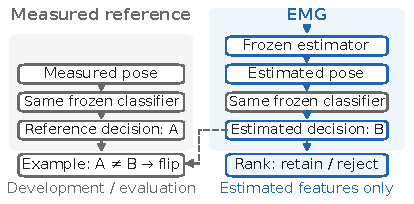
\includegraphics[width=\linewidth]{figures/fig1_compact.pdf}
\caption{Evaluating input substitution without changing the downstream classifier. Measured and EMG-estimated poses are passed through the same frozen consumer. Their decisions are compared offline to identify flips, while the selection scorer ranks estimated-input decisions without access to the measured-pose reference.}
\label{fig:substitution}
\end{figure}

\subsection{Decision Fidelity, Coverage, and Reference-Class Support}\label{decision-fidelity-coverage-and-reference-class-support}
For a paired block, suppose the frozen classifier outputs A from measured pose and B from estimated pose. If A and B differ, the block is counted as a flip. Measured pose is needed to identify flips during development and offline evaluation, but is not available to the selection scorer when ranking inputs.

For consumer \(i\), participant \(u\), and block \(t\), measured pose \(q_{u,t}\) and estimated pose \(\hat q_{u,t}\) define
\begin{equation}\label{eq:flip}
F_{u,t}^{(i)}=\mathds{1}\!\left[C_i(\hat q_{u,t})\neq C_i(q_{u,t})\right].
\end{equation}

We evaluate selection in two ways. Overall disagreement (U) is the proportion of retained, reference-valid blocks whose decisions differ. Coverage is the proportion of prediction-valid blocks retained.

Let \(V_u\) contain prediction-valid blocks, \(P_u\subseteq V_u\) those also having valid measured references, and \(A_u\subseteq V_u\) accepted blocks (consumer/method indices suppressed).
\begin{equation}\label{eq:overall}
U_u^{(i)}=\frac{\sum_{t\in A_u\cap P_u}F_{u,t}^{(i)}}{|A_u\cap P_u|},
\qquad
\gamma_u=\frac{|A_u\cap V_u|}{|V_u|}.
\end{equation}
Overall disagreement is undefined if \(A_u\cap P_u=\varnothing\). Missing-reference blocks contribute to coverage, but not to the observed disagreement denominator.

The reference-class support set is
\begin{equation}\label{eq:reference-support}
R_{u,k}^{(i)}=\left\{t\in P_u:C_i(q_{u,t})=k\right\}.
\end{equation}

Class-balanced disagreement (B) first calculates disagreement within each fixed measured-pose reference class and then averages those class rates equally. B is reported only when all fixed reference classes have at least 30 reference-valid blocks before selection and at least 30 retained blocks afterward. Otherwise B is undefined; unsupported classes are never silently excluded.

\begin{equation}\label{eq:balanced}
B_u^{(i)}=\frac{1}{K_i}\sum_{k=1}^{K_i}
\frac{\sum_{t\in A_u\cap R_{u,k}^{(i)}}F_{u,t}^{(i)}}
{|A_u\cap R_{u,k}^{(i)}|}.
\end{equation}

\subsection{Selective Scoring Methods}\label{selective-scoring-methods}
Selection changes which estimated-input decisions are retained, not the classes predicted by the frozen consumer. We compare three ranking strategies. Boundary ranks inputs by their distance from the consumer's nearest competing decision boundary. Score-only uses the consumer's predicted class, discriminant scores, score gap, entropy, and boundary distance to learn flip risk. Full adds estimated-pose information and descriptors of variation across fixed EMG input views.

For each consumer, the learned scorers are trained using paired development recordings with measured-pose flip labels. The primary overall-risk configuration uses histogram gradient boosting and is denoted Score-only/U or Full/U. A separate class-weighted configuration uses logistic regression to study balanced-risk training. During evaluation, all ranking features come from the estimated-input pathway; measured pose is used only to score the retrospective outcome.

Full includes eight pose angles, source-fitted Fisher coordinates, and two descriptors from four fixed EMG views: original, 0.97/1.03 amplitude scaling, and deterministic Gaussian noise at 0.005 times whole-record RMS. Fitting uses up to 5000 deterministically sampled paired blocks per participant, with equal participant and within-participant flip-state weights for /U. Histogram gradient boosting uses 100 iterations, depth 3, learning rate 0.1, L2 penalty 1, and seed 0. The balanced configuration uses reference-class/flip-state weighting and standardized logistic regression (\(C=1\), 300 iterations, seed 0).



\subsection{Selection and Evaluation Protocols}\label{selection-and-evaluation-protocols}
Our primary analysis compares methods at equal offline retention budgets. For each participant, inputs are ranked using estimated-input features and the top 10\%, 30\%, 50\%, or 70\% of prediction-valid blocks are retained, with deterministic tie handling. No Gate retains all prediction-valid blocks. Retention is defined on prediction-valid blocks, whereas disagreement requires valid paired references.

Because each participant is ranked using their own full-record score distribution, this protocol measures retrospective ranking rather than a deployable common threshold. A separate development-selected fixed-threshold audit evaluates whether predefined disagreement and coverage requirements can be met without choosing thresholds on the evaluation cohort.

Nineteen development participants comprise 13 fitting, three threshold-selection, and three diagnostic-validation participants. Validation affects neither fitting nor threshold selection. Stable score ordering with fixed file/block order resolves ties; a budget \(r\) retains \(\lceil r|V_u|\rceil\) blocks. Threshold feasibility requires disagreement \(\leq10\%\) for every threshold-development participant and median coverage \(\geq10\%\); the balanced objective also requires complete class support. Infeasible settings use the prespecified 30\% diagnostic fallback without being counted as feasible.

\subsection{Cohorts and Statistical Analysis}\label{cohorts-and-statistical-analysis}
The two previously examined evaluation cohorts comprise A20 (20 participants; 1,650,789 valid measured--estimated pairs) and N80 (80 participants; 7,111,408 pairs). They are analyzed separately and are not treated as independent confirmation after repeated examination. Participants used for selection-scorer development are separate from the reported evaluation participants; this separation does not certify the upstream estimator's training membership.

The exact training records associated with the released upstream checkpoint could not be established. Public training metadata contain train records for 70 of 80 N80 participants and 16 of 20 A20 participants, but metadata overlap does not by itself prove exposure of the actual checkpoint. We therefore make no verified upstream unseen-participant generalization claim.

Participants, not blocks, are the statistical units. Method differences are calculated within each participant before taking the median. Descriptive 95\% intervals for paired median effects use 10,000 participant-level bootstrap resamples. Consumers and retention budgets share participants and are dependent comparisons; the intervals are pointwise descriptive summaries rather than family-wise simultaneous confidence statements. Balanced comparisons use only jointly evaluable participants and report their counts.

% Reproducibility detail: deterministic cohort/participant-list bootstrap seeds are recorded in the sealed analysis code. The table caption distinguishes paired effects from separate medians.



\section{RESULTS}\label{results}
\begin{table*}[!b]
\centering
\caption{Overall decision disagreement in N80 at 30\% offline retention. The final column reports the median within-participant reduction relative to Boundary and its pointwise 95\% bootstrap interval (pp; n=80). The method columns contain separately calculated participant medians (\%).}
\label{tab:overall}
\begingroup
\small
\setlength{\tabcolsep}{3pt}
\renewcommand{\arraystretch}{1.05}
\begin{tabular}{lrrrrl}
\toprule
Consumer & No Gate $U$ & Boundary $U$ & Score-only/U $U$ & Full/U $U$ & Paired Boundary--Full/U (95\% CI)\\
\midrule
DB9 posture & 38.91 & 21.95 & 17.29 & 16.00 & 4.651 [2.784, 6.505]\\
DB9 grasp & 18.37 & 6.67 & 4.87 & 3.46 & 1.867 [1.431, 2.371]\\
CeTI posture & 43.05 & 24.73 & 21.87 & 20.77 & 3.973 [2.918, 5.312]\\
CeTI grasp & 41.10 & 31.59 & 29.60 & 25.65 & 4.261 [2.214, 6.446]\\
SHOW instruction & 16.43 & 6.93 & 6.29 & 4.10 & 2.591 [1.655, 3.006]\\
KIN phase & 22.32 & 5.95 & 3.81 & 3.66 & 2.107 [1.300, 3.302]\\
\bottomrule
\end{tabular}
\par\smallskip
\begin{minipage}{\linewidth}\footnotesize
No Gate retains all prediction-valid blocks; selective methods retain 30\%. $U$: participant medians (\%; lower is better). Paired effects: percentage points (higher is better). Intervals are pointwise descriptive participant-bootstrap summaries, not differences between method medians.
\end{minipage}
\endgroup

\end{table*}

\begin{figure*}[!b]
\centering
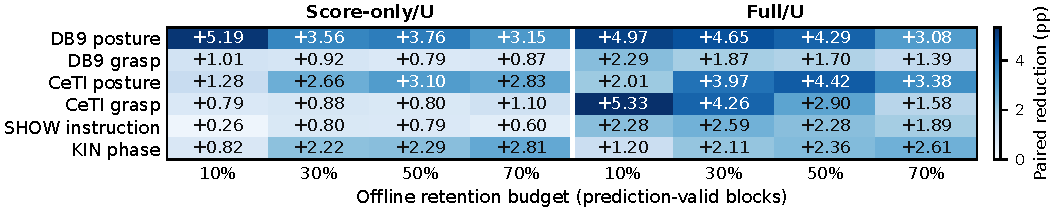
\includegraphics[width=\linewidth]{figures/fig2_N80_ranking.pdf}
\caption{Median paired reductions in overall decision disagreement relative to Boundary across six frozen consumers and four matched offline retention budgets in N80. Positive values indicate lower disagreement under learned ranking. The comparisons share participants and should not be interpreted as independent replications.}
\label{fig:ranking}
\end{figure*}
\subsection{Decision Disagreement Under Pose Substitution}\label{decision-disagreement-under-pose-substitution}
Pose substitution changed decisions for every frozen consumer. Without rejection, N80 participant-median disagreement ranged from 16.43\% for SHOW instruction to 43.05\% for CeTI posture (Table~\ref{tab:overall}). The variation shows that different consumers can respond differently to the same paired target pose inputs.


Reference-class support was already uneven before selection. All fixed classes met the predefined minimum in 22/80 participants for DB9 posture and 79/80 for KIN phase, versus 80/80 for the other four consumers. These differences matter when interpreting class-balanced outcomes after rejection.

\subsection{Selective Ranking Across Frozen Consumers}\label{selective-ranking-across-frozen-consumers}
Full/U ranking reduced overall disagreement across all six consumers in N80 at 30\% offline retention. Relative to Boundary, the median within-participant reduction ranged from 1.867 percentage points for DB9 grasp (95\% descriptive bootstrap interval: 1.431--2.371) to 4.651 points for DB9 posture (2.784--6.505). All six pointwise intervals were above zero (Table~\ref{tab:overall}).

Across the four tested retention budgets, Full/U showed positive median paired improvements over Boundary in all 24 consumer--budget comparisons within each of A20 and N80 (Fig.~\ref{fig:ranking}). These comparisons share participants and related experimental conditions, so the direction counts are descriptive rather than independent confirmations.

The learned Score-only/U control also improved disagreement relative to Boundary. Direct paired comparisons favored Full/U over Score-only/U in 23/24 N80 and 22/24 A20 consumer--budget settings, with non-improving conditions retained in the analysis. At 30\% retention, the largest reported N80 paired Full/U-versus-Score-only/U improvement was 3.79 points for CeTI grasp.



% Auxiliary feature and threshold results integrated into Results B (reader revision).
Feature-group ablations showed that the gain from richer scoring features depended on the consumer. Conditional gains from the fixed-view augmentation descriptors were smaller, ranging from 0.040 to 0.226 points across the six consumers at 30\% retention. Four of the six pointwise intervals for this augmentation contrast included zero. These analyses were exploratory on previously examined cohorts and did not change the original Full/U models.

Fixed-threshold feasibility was more limited than offline ranking performance: 4/24 auxiliary Score-only configurations passed their predefined criteria, with none of the 12 balanced-targeted configurations passing. Original Full development-selected threshold feasibility was 3/6 under the overall-risk objective and 0/6 under the balanced-risk objective.



\begin{figure*}[!t]
\centering
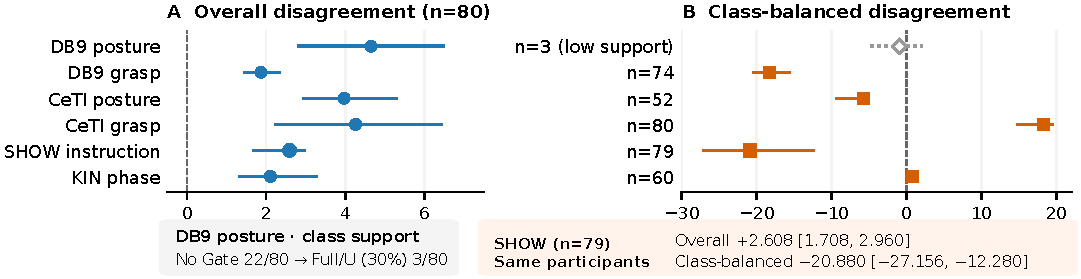
\includegraphics[width=\linewidth]{figures/fig3_class_fidelity.pdf}
\caption{Overall improvements do not guarantee class-balanced improvements. Paired Boundary-Full/U disagreement reductions at 30\% offline retention are shown for overall (A) and class-balanced (B) outcomes. Positive values indicate improvement; negative values indicate worsening. Overall effects use 80 participants, whereas balanced effects require complete support under both methods and use the indicated participant counts. SHOW retains opposite effect directions when both measures are evaluated in the same 79 participants. DB9 posture has only three jointly evaluable participants for the balanced comparison.}
\label{fig:fidelity}
\end{figure*}

\subsection{Class-Conditional Disagreement and Reference Support}\label{sec:classconditional}
The next question is whether this overall improvement also preserves decisions across reference classes. At 30\% offline retention, Full/U reduced overall disagreement relative to Boundary across all six consumers, but class-balanced outcomes varied (Fig.~\ref{fig:fidelity}).

SHOW instruction revealed a clear trade-off. Among the same 79 participants with complete reference-class support, Full/U reduced overall disagreement by a median of 2.608 percentage points (95\% descriptive bootstrap interval: 1.708--2.960), while class-balanced disagreement increased by 20.880 points (12.280--27.156). Thus, an aggregate improvement coincided with substantially worse class-balanced performance within the same participants. In contrast, CeTI grasp improved both overall and class-balanced disagreement by 4.261 and 18.31 points, respectively, with all 80 participants evaluable.

Selection also reduced the number of participants for whom class-balanced disagreement could be evaluated. For DB9 posture, complete reference-class support was available in 22 of 80 participants without rejection, but only three under Full/U at 30\% retention. Its class-balanced comparison therefore describes only three jointly evaluable participants, not the full cohort. Together, these findings show why overall disagreement, class-balanced disagreement, and reference-class support must be interpreted jointly.



\section{DISCUSSION}\label{discussion}
A shared pose interface must be judged by the decisions it preserves, as well as by the format of the input it accepts. The results show that input compatibility alone does not guarantee preserved decisions across independently trained pose consumers. Overall-risk ranking improved decision agreement in the evaluated settings, but it did not ensure that each measured-pose reference class benefited equally.

Evaluating only aggregate disagreement would miss both problems.

The interpretation is deliberately limited. A flip compares two decisions of the same frozen classifier, not either decision against an independently labeled target action. Joint selections, data calibration procedures, and block indexing were examined, but cross-source absolute pose equivalence and independent residual synchronization were not established. The upstream checkpoint's actual training membership also remains unresolved despite overlap with public training metadata. Finally, whole-record processing and participant-specific retrospective ranking do not validate a causal online rejection system.



\section{CONCLUSION}\label{conclusion}
Replacing measured hand pose with EMG-estimated pose changed the decisions of six frozen pose consumers. Learned offline ranking reduced overall disagreement relative to boundary-based selection, but these gains did not guarantee class-balanced improvement or sufficient reference-class support. The findings show that downstream decision fidelity should be assessed jointly through overall disagreement, class-balanced disagreement, and evaluable class support. This is evidence about specified frozen interfaces under retrospective evaluation, not a claim of target-task correctness or online deployment reliability.

% INTERNAL TODO: Code Availability may be inserted only after the actual
% public release URL/tag and the 2027 link/anonymity rules are verified.
% No publication statement is printed in this draft.
